%  ----------------------------------------------------------------------------
%
%       Copyright (for the thesis) 2009 by [author - insert yourself]
%
%       This thesis is published under the
%       Creative Commons Attribution-No Derivative Works 3.0 Austria License
%       as detailed at http://creativecommons.org/licenses/by-nd/3.0/at/
%
%  ----------------------------------------------------------------------------
%  Template credits and license:
%  ----------------------------------------------------------------------------
%
%       "Fakultät für Informatik" diploma/master thesis template 2008
%
%       based upon "Diploma thesis template 2005" by lukas.silberbauer(at)gmx.at
%       based upon "Diplomarbeit mit LaTeX" by Tobias Erbsland
%       incorporating a title page by Informatik-Forum user "Baby"
%       polished and ported to the TU fonts package by Jakob Petsovits
%
%       published under the terms of
%
%  ----------------------------------------------------------------------------
%  "THE BEER-WARE LICENSE":
%  <lukas.silberbauer(at)gmx.at> wrote this file. As long as you retain this
%  notice you can do whatever you want with this stuff. If we meet some day,
%  and you think this stuff is worth it, you can buy me (us) a beer in return.
%  ----------------------------------------------------------------------------
%
%  (end of template credits)
%

%
% Variablen, die fürs Deckblatt verwendet werden.
% Die grobe Dokumentenstruktur findet sich übrigens ganz unten in dieser Datei.
%
\newcommand{\thesistype}{MASTERARBEIT}
\newcommand{\thesistitle}{Effektivit\"{a}tsanalyse des c-Collision Protokolls}
\newcommand{\thesissubtitle}{ als gewichteter Datenbalancierer in einem parallelen Out-of-Core Renderer.}

\newcommand{\thesisauthor}{Timo Wiesemann}
\newcommand{\matrikelnr}{6015295}
\newcommand{\zuerlangendertitel}{Diplom-Informatiker}
\newcommand{\studium}{Software Engineering \& Internet Computing}

\newcommand{\institut}{Institut f\"{u}r rechnergest\"{u}tzte Sprachengraphik- und Wirkungsinteraktivit\"{a}t}
\newcommand{\institutsuni}{Johannes Kepler Universit\"{a}t Linz} % disabled by default
\newcommand{\betreuer}{o.Univ.Prof. Dipl.-Ing. Dr. Dr.h.c.mult. Montgomery Burns}
\newcommand{\assistent}{Univ.-Ass. Dr. Waylon Smithers}

%
% Globale Weichenstellungen fürs ganze Dokument.
%
\documentclass[%
  pdftex,%              PDFTex verwenden
  a4paper,%             A4 Papier
  oneside,%             Einseitig
  bibtotocnumbered,%    Literaturverzeichnis nummeriert einfügen
  idxtotoc,%            Index ins Verzeichnis einfügen
  halfparskip,%         Europäischer Satz mit abstand zwischen Absätzen
  chapterprefix,%       Kapitel anschreiben als Kapitel
  %headsepline,%         Linie nach Kopfzeile
  %footsepline,%         Linie vor Fusszeile
  12pt%                 Größere Schrift, besser lesbar am Bildschrim
]{scrbook}


%
% Paket für die Indexerstellung.
%
\usepackage{makeidx}

%
% Paket für Übersetzungen ins Deutsche
%
\usepackage[german, english]{babel}

%
% Paket, um \today auch im Format dd.mm.yyyy anzeigen zu können
%  (für die Titelseite, mit \numdate)
%
\usepackage[german]{isodate}

%
% Pakete um Latin1 Zeichnensätze verwenden zu können und die dazu
%  passenden Schriften.
%
%\usepackage{ucs}
\usepackage[utf8]{inputenc}
\usepackage[T1]{fontenc}

%
% Paket zum Erweitern der Tabelleneigenschaften
%
\usepackage{array}

%
% Paket um Grafiken einbetten zu können
%
\usepackage{graphicx}


%
% Zeilenabstand einstellen
%
\usepackage{setspace}
\onehalfspacing
%\doublespacing


%\setlength{\baselineskip}{24pt}
%\renewcommand{\baselinestretch}{1.5}


%
% define variables
%
\def\maintitle#1{\gdef\maintitle{#1}}
\def\subtitle#1{\gdef\subtitle{#1}}

%
% Zeilenumbruch bei Bildbeschreibungen.
%
\setcapindent{1em}

%
% kopf und fusszeilen
%
\pagestyle{headings}

%
% mathematische symbole aus dem AMS Paket.
%
\usepackage{amsmath}
\usepackage{amssymb}

%
% Type 1 Fonts für bessere darstellung in PDF verwenden.
%
\usepackage{mathptmx}           % Times + passende Mathefonts
%\usepackage[scaled=.92]{helvet} % skalierte Helvetica als \sfdefault
\usepackage{courier}            % Courier als \ttdefault
\usepackage{tufonts}            % TU-Schriften als \sfdefault

%
% Spezielle Schrift verwenden.
%
\renewcommand{\encodingdefault}{T1}
\renewcommand{\familydefault}{\rmdefault}
\renewcommand{\bfdefault}{db}   % bold would be too bold, use demibold instead
\renewcommand{\mddefault}{l}    % use TU Light, looks better than medium weight



%
% Paket um Textteile drehen zu können
%
\usepackage{rotating}


%
% Für Acronyme
%
\usepackage{acronym}

%
% Package für Farben im PDF
%
\usepackage{color}

%
% Paket für Links innerhalb des PDF Dokuments
%
\definecolor{LinkColor}{rgb}{0,0,0.5}

\usepackage[
pdfauthor={\thesisauthor},
bookmarks=true, % PDF bookmarks allowed. NB! The level depth of bookmarks is the same as in the TOC.
unicode=true, % PDF bookmarks in Unicode.
bookmarksnumbered=true, % Section numbers in PDF bookmarks.
bookmarksopenlevel=1, % The open level in PDF bookmarks.
hyperindex=true, % Hyperlinked index.
plainpages=false, % Name arabic and roman page numbers differently.
colorlinks=true, % Links are marked as coloured text, not coloured box.
linkcolor=linkc, % The colour for in-document links (e.g. in the table of contents).
citecolor = citec, % The colour for bibliographic citations.
urlcolor=urlc, % The colour for hyperlinks to the Net.
pdfpagelayout=OneColumn % Continuous page scrolling.
]{hyperref}
\hypersetup{
  colorlinks=true,
  linkcolor=LinkColor,
  citecolor=LinkColor,
  filecolor=LinkColor,
  menucolor=LinkColor,
  pagecolor=LinkColor,
  urlcolor=LinkColor
}

%
% Paket um Listings sauber zu formatieren.
%
\usepackage[savemem]{listings}
\lstloadlanguages{TeX}

%
% ---------------------------------------------------------------------------
% Listing Definitionen für PHP Code
%
\definecolor{lbcolor}{rgb}{0.85,0.85,0.85}
\lstset{language=[LaTeX]TeX,
  numbers=left,
  stepnumber=1,
  numbersep=5pt,
  numberstyle=\tiny,
  breaklines=true,
  breakautoindent=true,
  postbreak=\space,
  tabsize=2,
  basicstyle=\ttfamily\footnotesize,
  showspaces=false,
  showstringspaces=false,
  extendedchars=true,
  backgroundcolor=\color{lbcolor}
}

% ---------------------------------------------------------------------------
% Neue Umgebungen
% ---------------------------------------------------------------------------

\newenvironment{ListChanges}%
  {\begin{list}{$\diamondsuit$}{}}%
  {\end{list}}

%
% Index erzeugen
%
\makeindex


%%%%%%%%%%%%%%%%%%%%%%%%%%%%%%%%%%%%%%%%%%%%%%%%%%%%%%%%%%%%%%%%%%%%%%
%
% Document structure
%
%%%%%%%%%%%%%%%%%%%%%%%%%%%%%%%%%%%%%%%%%%%%%%%%%%%%%%%%%%%%%%%%%%%%%%

\begin{document}

\pagenumbering{alph}
%  ----------------------------------------------------------------------------
%
%       Copyright (for the thesis) 2009 by [author - insert yourself]
%
%       This thesis is published under the
%       Creative Commons Attribution-No Derivative Works 3.0 Austria License
%       as detailed at http://creativecommons.org/licenses/by-nd/3.0/at/
%
%  ----------------------------------------------------------------------------
%  Template credits and license:
%  ----------------------------------------------------------------------------
%
%       "Fakultät für Informatik" diploma/master thesis template 2008
%
%       based upon "Diploma thesis template 2005" by lukas.silberbauer(at)gmx.at
%       based upon "Diplomarbeit mit LaTeX" by Tobias Erbsland
%       incorporating a title page by Informatik-Forum user "Baby"
%       polished and ported to the TU fonts package by Jakob Petsovits
%
%       published under the terms of
%
%  ----------------------------------------------------------------------------
%  "THE BEER-WARE LICENSE":
%  <lukas.silberbauer(at)gmx.at> wrote this file. As long as you retain this
%  notice you can do whatever you want with this stuff. If we meet some day,
%  and you think this stuff is worth it, you can buy me (us) a beer in return.
%  ----------------------------------------------------------------------------
%
%  (end of template credits)
%

\selectlanguage{german}
\begin{titlepage}
\parskip0pt
\fontfamily{fts}\selectfont

\vspace*{-0.75cm}

\hbox to \hsize{
\includegraphics[scale=0.75]{images/Logo_Uni_Paderborn.pdf}\hss}
 % Logo_Uni_Paderborn.pdf: 442x117 pixel, 72dpi, 15.59x4.13 cm, bb=0 0 442 117

\vspace{1.2cm}

\begin{center}
\begin{Large}\thesistype \end{Large}\vspace{1cm}
 
\dmseries

\huge{

Effektivit\"{a}tsanalyse

des \textit{c}-Collision Protokolls

\hbox to \hsize{\hss als gewichteter Datenbalancierer\hss}

in einem parallelen

Out-of-Core Renderer
} 
\end{center}

\vfill

\begin{center}
\begin{Large}\dmseries\thesisauthor\end{Large} 


\end{center}

% 2. Seite...

\newpage~\newpage
\thispagestyle{empty}

\parskip12pt

\begin{center}
  \begin{Large}\thesistype \end{Large}  


  \begin{normalsize}DPO4 \end{normalsize} \bigskip 


  \vspace{2.0cm}
  \begin{normalsize}Vorgelegt von: \end{normalsize} 


  \begin{Large}\dmseries\thesisauthor\end{Large} 


  \begin{normalsize}Matrikelnummer: \matrikelnr\end{normalsize} \bigskip


  \vspace{1.0cm}
  \begin{normalsize}Vorgelegt bei: \end{normalsize} 


  \begin{large}\dmseries Dr. Matthias Fischer\end{large} 


  \begin{large}\dmseries Prof. Gitta Domik\end{large}\bigskip 


  \begin{normalsize}Betreuer: \end{normalsize} 


  \begin{large}\dmseries Dipl.-Inform. Tim S\"{u}\ss\end{large} \bigskip


  \vspace{3.0cm}
  \begin{normalsize}\institut\end{normalsize}\\
  \begin{normalsize}\institutsuni\end{normalsize}\bigskip 


  \begin{normalsize}Paderborn, im Februar 2010\end{normalsize}

\end{center}
\end{titlepage}
\newpage~\newpage
%
% EOF
%


\selectlanguage{english}
\pagenumbering{roman}
\setcounter{page}{1}

%  ----------------------------------------------------------------------------
%
%       Copyright (for the thesis) 2009 by [author - insert yourself]
%
%       This thesis is published under the
%       Creative Commons Attribution-No Derivative Works 3.0 Austria License
%       as detailed at http://creativecommons.org/licenses/by-nd/3.0/at/
%
%  ----------------------------------------------------------------------------
%  Template credits and license:
%  ----------------------------------------------------------------------------
%
%       "Fakultät für Informatik" diploma/master thesis template 2008
%
%       based upon "Diploma thesis template 2005" by lukas.silberbauer(at)gmx.at
%       based upon "Diplomarbeit mit LaTeX" by Tobias Erbsland
%       incorporating a title page by Informatik-Forum user "Baby"
%       polished and ported to the TU fonts package by Jakob Petsovits
%
%       published under the terms of
%
%  ----------------------------------------------------------------------------
%  "THE BEER-WARE LICENSE":
%  <lukas.silberbauer(at)gmx.at> wrote this file. As long as you retain this
%  notice you can do whatever you want with this stuff. If we meet some day,
%  and you think this stuff is worth it, you can buy me (us) a beer in return.
%  ----------------------------------------------------------------------------
%
%  (end of template credits)
%

\addchap{Abstract}

Describes the contents of this thesis in significantly less than a single page.
To quote the insightful words in chapter~\ref{conclusion}, % "~" is a &nbsp;

Bla Bla Bla Bla Bla Bla Bla Bla Bla Bla Bla Bla Bla Bla Bla Bla Bla Bla Bla Bla
Bla Bla Bla Bla Bla Bla Bla Bla Bla Bla Bla Bla Bla Bla Bla Bla Bla Bla Bla Bla
Bla Bla Bla Bla Bla Bla Bla Bla Bla Bla Bla Bla Bla Bla Bla Bla Bla Bla Bla Bla
Bla Bla Bla Bla Bla Bla Bla Bla Bla Bla Bla Bla Bla Bla Bla Bla Bla Bla Bla Bla
Bla Bla Bla Bla Bla Bla Bla Bla Bla Bla Bla Bla Bla Bla Bla Bla Bla Bla Bla Bla
Bla Bla Bla Bla Bla Bla Bla Bla Bla Bla Bla Bla Bla Bla Bla Bla Bla Bla Bla Bla
Bla Bla Bla Bla Bla Bla Bla Bla Bla Bla Bla Bla Bla Bla Bla Bla Bla Bla Bla Bla
Bla Bla Bla Bla Bla Bla Bla Bla Bla Bla Bla Bla Bla Bla Bla Bla Bla Bla Bla Bla
Bla Bla Bla Bla Bla Bla Bla Bla Bla Bla Bla Bla Bla Bla Bla Bla Bla Bla Bla Bla
Bla Bla Bla Bla Bla Bla Bla Bla Bla Bla Bla Bla Bla Bla Bla Bla Bla Bla Bla Bla
Bla Bla Bla Bla Bla Bla Bla Bla

\addchap{Zusammenfassung}

Beschreibt den Inhalt der Arbeit in weit weniger als einer Seite.
Wie Kapitel~\ref{conclusion} so schön zu sagen pflegt: % "~" ist ein &nbsp;

Bla Bla Bla Bla Bla Bla Bla Bla Bla Bla Bla Bla Bla Bla Bla Bla Bla Bla Bla Bla
Bla Bla Bla Bla Bla Bla Bla Bla Bla Bla Bla Bla Bla Bla Bla Bla Bla Bla Bla Bla
Bla Bla Bla Bla Bla Bla Bla Bla Bla Bla Bla Bla Bla Bla Bla Bla Bla Bla Bla Bla
Bla Bla Bla Bla Bla Bla Bla Bla Bla Bla Bla Bla Bla Bla Bla Bla Bla Bla Bla Bla
Bla Bla Bla Bla Bla Bla Bla Bla Bla Bla Bla Bla Bla Bla Bla Bla Bla Bla Bla Bla
Bla Bla Bla Bla Bla Bla Bla Bla Bla Bla Bla Bla Bla Bla Bla Bla Bla Bla Bla Bla
Bla Bla Bla Bla Bla Bla Bla Bla Bla Bla Bla Bla Bla Bla Bla Bla Bla Bla Bla Bla
Bla Bla Bla Bla Bla Bla Bla Bla Bla Bla Bla Bla Bla Bla Bla Bla Bla Bla Bla Bla
Bla Bla Bla Bla Bla Bla Bla Bla Bla Bla Bla Bla Bla Bla Bla Bla Bla Bla Bla Bla
Bla Bla Bla Bla Bla Bla Bla Bla Bla Bla Bla Bla Bla Bla Bla Bla Bla Bla Bla Bla
Bla Bla Bla Bla Bla Bla Bla Bla

%
% EOF
%

%  ----------------------------------------------------------------------------
%
%       Copyright (for the thesis) 2009 by [author - insert yourself]
%
%       This thesis is published under the
%       Creative Commons Attribution-No Derivative Works 3.0 Austria License
%       as detailed at http://creativecommons.org/licenses/by-nd/3.0/at/
%
%  ----------------------------------------------------------------------------
%  Template credits and license:
%  ----------------------------------------------------------------------------
%
%       "Fakultät für Informatik" diploma/master thesis template 2008
%
%       based upon "Diploma thesis template 2005" by lukas.silberbauer(at)gmx.at
%       based upon "Diplomarbeit mit LaTeX" by Tobias Erbsland
%       incorporating a title page by Informatik-Forum user "Baby"
%       polished and ported to the TU fonts package by Jakob Petsovits
%
%       published under the terms of
%
%  ----------------------------------------------------------------------------
%  "THE BEER-WARE LICENSE":
%  <lukas.silberbauer(at)gmx.at> wrote this file. As long as you retain this
%  notice you can do whatever you want with this stuff. If we meet some day,
%  and you think this stuff is worth it, you can buy me (us) a beer in return.
%  ----------------------------------------------------------------------------
%
%  (end of template credits)
%

\addchap{Acknowledgements}

I would like to dedicate this thesis to (...) who (...). Bla bla, etc.

I wish to acknowledge (...) for (...). Kudos go out to (...).

I thank Prof. (...) for the supervision of this thesis.

To the Free Software / Open Source communities, I extend my gratitude for
making all of my work worthwhile -- it's just so much more fun if there is
someone out there who can put the results into productive use.

\clearpage

%
% EOF
%


\tableofcontents
\listoffigures
\listoftables

\pagenumbering{arabic}
\setcounter{page}{1}

%  ----------------------------------------------------------------------------
%
%       Copyright (for the thesis) 2009 by [author - insert yourself]
%
%       This thesis is published under the
%       Creative Commons Attribution-No Derivative Works 3.0 Austria License
%       as detailed at http://creativecommons.org/licenses/by-nd/3.0/at/
%
%  ----------------------------------------------------------------------------
%  Template credits and license:
%  ----------------------------------------------------------------------------
%
%       "Fakultät für Informatik" diploma/master thesis template 2008
%
%       based upon "Diploma thesis template 2005" by lukas.silberbauer(at)gmx.at
%       based upon "Diplomarbeit mit LaTeX" by Tobias Erbsland
%       incorporating a title page by Informatik-Forum user "Baby"
%       polished and ported to the TU fonts package by Jakob Petsovits
%
%       published under the terms of
%
%  ----------------------------------------------------------------------------
%  "THE BEER-WARE LICENSE":
%  <lukas.silberbauer(at)gmx.at> wrote this file. As long as you retain this
%  notice you can do whatever you want with this stuff. If we meet some day,
%  and you think this stuff is worth it, you can buy me (us) a beer in return.
%  ----------------------------------------------------------------------------
%
%  (end of template credits)
%

\chapter{Einleitung}

\begin{itemize}
 \item Was habe ich gemacht?
 \item Zusammenfassung vorweggenommen
 \item c-Collision Protokoll nicht vergessen!
\end{itemize}

\section{Motivation}
\label{introduction:motivation}

\begin{itemize}
 \item Herausforderung
 \item Grafikkarten
 \item 3D-Modelle
 \item OutOfCore
 \item im Netzwerk
 \item Hybrides System
 \item Datenmenge
 \item Format
 \item Cluster-Konfiguration
\end{itemize}

Considering \cite{wilcox}, we follow that ... blah, blah ... so that it becomes
clear that ... blah, blah ... upon which we may safely assume that Wilcox is
actually correct in his reasoning, and by investigating ... blah, blah ...
we hope to gain detailed insight into this topic.

-


%
% EOF
%

\chapter{Grundlagen}
\label{chap:basics}
\todo[size=\small, inline, color=yellow]{Grundlagen $\rightarrow$ Spellcheck!}
\todo[size=\small, inline]{Evtl. besseren Namen für Kapitel "`Grundlagen"' finden $\rightarrow$ Grundlegende Algorithmen/Techniken?!}%
\textbf{Hier kommt nur rein was ICH mache!}\\
An dieser Stelle soll zunächst ein Überblick über die in der vorliegenden Arbeit verwendeten Techniken gegeben werden. Diese beinhalten unter anderem Algorithmen der Computergrafik, welche Datenstrukturen benutzt werden und wie die Speicherverwaltung organisiert ist.

\section{Datenstrukturen}
\label{sec:basics:datenstrukturen}
\textbf{Wofür und warum?!}\\
3D-Modelle aus Computer Aided Design - Anwendungen (CAD) werden üblicherweise nach ihrer Funktion gruppiert. Das mag beim Entwurf solcher Systeme auch praktisch sein, bei der Visualisierung kann dies jedoch zu Problemen führen. Bei CAD-Modellen in Größenordnung der Boeing 777\footnote{\todo[size=\small, inline]{Boeing Herkunftshinweis verschieben an die erste Stelle wo es erwähnt wird.}%
Das 3D-Modell der Boeing 777 wurde freundlicherweise zur Verfügung gestellt von The Boeing Company, Seattle, WA, USA.} (ca. 350 Millionen Dreiecke) ist es wichtig, dass diese in eine geeignete räumliche Unterteilung überführt werden. Da ein Out-Of-Core-Renderer entwickelt wurde, findet ein ständiges Laden und Verwerfen von Teilmodellen statt. Je länger ein Renderer benötigt um herauszufinden, welche Teile des Modells er verwerfen kann und welche er als erstes anfordern sollte, desto länger braucht er auch um ein Bild zu erstellen. In dieser Arbeit wurde als hierarchische räumliche Unterteilung ein Randomized Sampletree (\ref{sec:basics:sampletree}) und zum Vergleich ein Loose Octree gewählt.

\subsection{Loose Octree}
\label{sec:basics:octree}
Um einen Octree\footnote{\cite{RTR3}, Seiten 647 ff.} zu Erzeugen wird die gesamte Szene in eine minimale Boundingbox eingeschlossen. Rekursiv wird diese Box entlang der drei räumlichen Achsen in der Mitte geteilt, woraus sich jeweils acht gleich-große Boundingboxen ergeben. Dieser Vorgang wird so lange wiederholt bis ein Haltekriterium erfüllt ist. Im Falle der Boeing wurde festgelegt, dass höchstens 5.000 Dreiecke in einer Box liegen dürfen und die maximale Tiefe des Baums wurde auf 14 beschränkt. Erfüllt ein Octree-Knoten eines dieser Kriterien, wird nicht weiter untereilt. Dementsprechend gibt es keine leeren Blatt-Knoten im Octree. In Abbildung \ref{fig:basics:octree} ist ein Octree zu sehen.\\
\begin{figure}
 \centering
  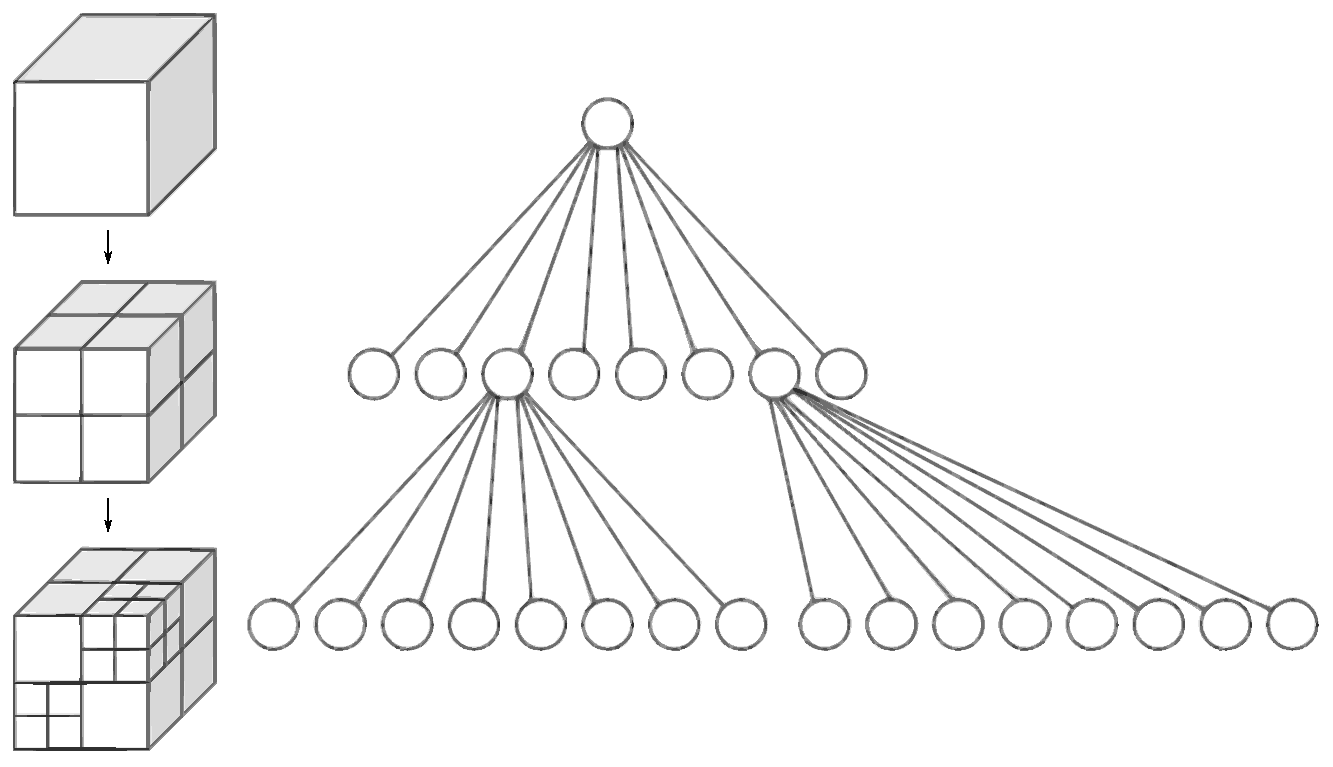
\includegraphics[scale=0.5]{images/octree.pdf}
 % octree.pdf: 640x368 pixel, 72dpi, 22.58x12.98 cm, bb=0 0 640 368
  \caption{Ein Octree der Tiefe 2. \textit{links: die räumliche Darstellung, rechts: die Baumdarstellung. Quelle: \htmladdnormallink{http://de.wikipedia.org/wiki/Octree}{http://de.wikipedia.org/wiki/Octree}}}
 \label{fig:basics:octree}
\end{figure}
In dieser Arbeit wurde jedoch eine spezielle Form des Octrees verwendet: der Loose Octree. Dieser erweitert den Octree um eine weitere Box pro Knoten: die sogenannte Loosebox. Sie teilt sich ihr Zentrum mit der Octree-Boundingbox, besitzt aber doppelte Kantenlängen. Wird nun festgestellt, dass in einem Knoten mehr als 5.000 Dreiecke liegen, wird die größe der einzelnen Dreiecke anhand der Loosebox geprüft. Liegt ein Dreieck vollständig in der Loosebox mit seinem Zentrum in der eigentlichen Boundingbox des Knotens, kann es weiter nach unten gereicht werden. Ist dies nicht der Fall, ist das Dreieck zu groß für den aktuellen Knoten und wird an den Vaterknoten gegeben (Abbildung \ref{fig:basics:looseoctree}).\\
Dies hat den Vorteil, dass große Dreiecke relativ weit oben im Baum zu liegen kommen und Kleinere entsprechend tief. Je größer ein Dreieck ist, desto größer ist auch die Wahrscheinlichkeit, dass das Dreieck sichtbar ist und somit gezeichnet werden muss. Bewegt man sich durch ein Modell, ist der Wurzelknoten, oder Szenen-Boundingbox, praktisch immer sichtbar, was bedeutet, dass die zur Wurzel gehörige Geometrie gezeichnet werden muss.
\begin{figure}
 \centering
  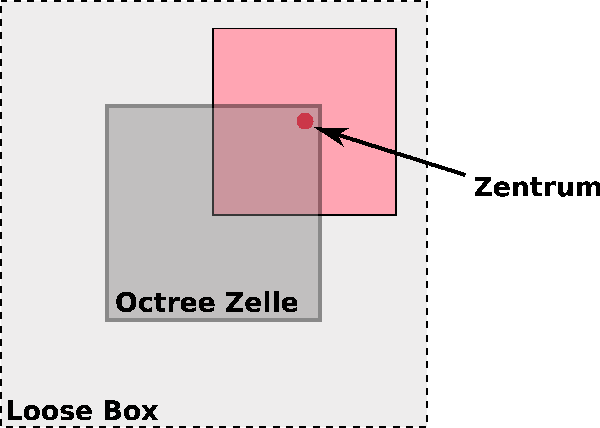
\includegraphics[scale=0.8]{images/looseoctree2.pdf}
  \caption{Ein Loose Octree in einer 2D-Darstellung. \textit{Das Zentrum des Objekts (rosa) befindet sich innerhalb der Octree Zelle, das gesamte Objekt befindet sich innerhalb der Loose Box. Quelle: nach \htmladdnormallink{http://anteru.net/2008/11/14/315/}{http://anteru.net/2008/11/14/315/}}}
 \label{fig:basics:looseoctree}
\end{figure}

\subsection{Randomized Sampletree}
\label{sec:basics:sampletree}
Als spezielle Ausprägung eines Loose Octrees gibt es den Randomized Sampletree \cite{klein}. Dieser unterschiedet sich von einem Octree darin, dass zufällig einzelne Dreiecke aus tieferen Knoten in höhere Knoten verschoben  wurden. Beim rendern der Szene wird in jedem Frame der Baum traversiert, um ein Frustum-Culling durchzuführen (siehe auch \ref{sec:basics:algos}). Ab einer bestimmten Tiefe im Baum wird die Traversion abgebrochen, um die Komplexität der Darstellung zu reduzieren. Dadurch kommt es allerdings zu Darstellungsfehlern, da nicht alle sichtbare Geometrie gerendert wird. An dieser Stelle schafft ein Randomized Sampletree abhilfe. Dadurch dass zufällige kleinere Dreiecke in höherliegenden Knoten gespeichert sind, werden diese auch gerendert. Ist die Flächensumme alle Dreiecke in einem Knoten des Sampletrees nicht größer als ein Pixel, wird die Traversion abgebrochen. Klein, Krokowski und Fischer \cite{klein} haben gezeigt, dass diese Geometrie-Approximation von weit entfernten Objekten durch zufällige Dreiecke eine hinreichend korrekte Darstellung liefert. Dieses Verfahren wurde für komplexe geometrische Umgebungen entwickelt, weshalb es in dieser Arbeit verwendet wurde.
\begin{figure}
 \centering
  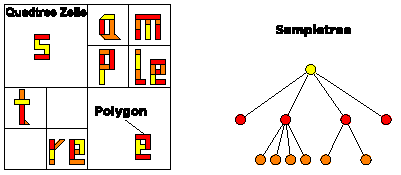
\includegraphics[scale=1.7]{images/sampletree2.pdf}
  \caption{Ein Sampletree in einer 2D-Darstellung. \textit{links: Eine Aufteilung von Polygonen in verschiedene Quadtree Zellen. rechts: Die Baumdarstellung des Sampletrees. Die farbigen Knoten geben an welche Polygonteile der linken Seite in welchen Knoten gespeichert wurden. Quelle: nach \cite{klein}}}
 \label{fig:basics:sampletree}
\end{figure}

\section{Computergrafik}
\label{sec:basics:computergrafik}
\todo[size=\small, inline]{Pipeline-Stall/Flush bei Farbsetzung muss nochmal gegengeprüft werden!}
Da Arbeitsspeicher in der Regel größer ist als der Speicher einer Grafikkarte, werden nicht alle geometrischen Objeke auf der Grafikkarte belassen. Wenn angeforderte Objekte bei einem Renderer eintreffen, werden die zunächst gar nicht an die Grafikkarte geschickt. Erst nach weiteren Tests, ob das Objekt immer noch sichtbar ist, findet der transfer zur GPU statt. Dort verbleiben sie dann, bis sie irgendwann aus platz- oder sichbarkeitsgründen verdrängt werden (siehe auch \ref{sec:basics:caching}). Um dies möglichst effizient umsetzen zu können werden Vertexbuffer Objects  (VBOs) genutzt. Die Idee ist dabei, dass Modelldaten, bestehend aus Vertices und Vertex-Normalen, in einem zusammenhängenden Speicherblock abgelegt werden. Ein Vertex besteht aus einer $xyz$-Koordinate und einer Vertex-Normalen. Der Zugriff auf Dreiecke erfolgt dann mittels einer Index-Liste, bei der immer drei Indices ein Dreieck ergeben. Alle Dreiecke eines Octree-Knotens wurden zu einem Vertexbuffer-Objekt zusammen gefasst (siehe \ref{sec:basics:octree}), da Geometrie innerhalb eines Knotens nicht weiter unterteilt wird. In Form von VBOs kann recht einfach entsprechender Platz im Grafik-RAM reserviert und die Daten in den Speicher geladen werden.\\
Im Gegensatz dazu verbleiben bei Vertex-Arrays alle Daten im Arbeitsspeicher des Rechners und werden für jeden Zeichenaufruf zur Grafikkarte übertragen. Vertex-Arrays bieten sich an, wenn Objekte nur einmal gezeichnet und dann verworfen werden. Von daher kommen sie nur auf den Datenknoten (siehe \ref{sec:impl:netzwerkarchitektur}) zum Einsatz, da diese ein getestetes Objekt nur in ihren Tiefenbuffer rendern und dann wieder verwerfen. Bei VBOs wäre der Overhead der Datenübertragung und der anschließenden Deallokation zu groß für eine einmalige Verwendung.
\begin{figure}
  \centering
  %%%%%%%%%%%%%%%%%%%%%%%%%%%%%%%%%%%%%%%%%%%%%%%%%%%%%%%%%
% 1D-Farbtextur mit Beschreibung und Labels
%%%%%%%%%%%%%%%%%%%%%%%%%%%%%%%%%%%%%%%%%%%%%%%%%%%%%%%%%


\begin{tikzpicture}
  \tikzset{ 
    every pin/.style={fill=yellow!50!white,rectangle,rounded corners=3pt,font=\small}, 
    small dot/.style={fill=black,circle,scale=0.3} } 
  \begin{axis}[
    x=13cm, y=1.0cm, 
    clip=false,
    ytick=\empty,
    xtick={0,0.03125,0.0625,0.09375,0.125,0.15625,0.1875,0.21875,0.25,0.28125,0.3125,
      0.34375,0.375,0.40625,0.4375,0.46875,0.5,0.53125,0.5625,0.59375,0.625,
      0.65625,0.6875,0.71875,0.75,0.78125,0.8125,0.84375,0.875,0.90625,0.9375,
      0.96875,1},
    xticklabels={$0$,$\frac{1}{n}$,$\frac{2}{n}$,$\frac{3}{n}$,$\frac{4}{n}$,$\frac{5}{n}$,$\frac{6}{n}$,$\frac{7}{n}$,$\frac{8}{n}$,$\frac{9}{n}$,$\frac{10}{n}$,
      $\frac{11}{n}$,$\frac{12}{n}$,$\frac{13}{n}$,$\frac{14}{n}$,$\frac{15}{n}$,$\frac{16}{n}$,$\frac{17}{n}$,$\frac{18}{n}$,$\frac{19}{n}$,$\frac{20}{n}$,
      $\frac{21}{n}$,$\frac{22}{n}$,$\frac{23}{n}$,$\frac{24}{n}$,$\frac{25}{n}$,$\frac{26}{n}$,$\frac{27}{n}$,$\frac{28}{n}$,$\frac{29}{n}$,$\frac{30}{n}$,
      $\frac{31}{n}$,$\frac{32}{n}$},
       %tickpos=right,
    major tick length={0.07cm},
    xtick align=outside,
    xtick pos=left,
    tick style={very thin, black},
    tick label style={
    font=\tiny},
    %major x tick num=5,
    %hide y axis,
    enlargelimits=false,
    axis on top] 
    \addplot graphics [xmin=0,xmax=1,ymin=0,ymax=1, 
      % trim=left bottom right top 
      includegraphics={trim=0 9 0 8,clip}
      ] 
      {images/colors.pdf}; 

\node[small dot,pin=-90:{$\frac{1}{2n}$}] at (axis description cs:0.017625,0) {}; 
%\node[small dot,pin=-45:{$\frac{1}{n}$}] at (axis description cs: 0.03325,0) {}; 

  \end{axis} 
\end{tikzpicture}

  \caption{1D-Farbtextur. $n=$Anzahl Farben. Um mittig auf den Texel der Farbe $i$ zuzugreifen, errechnet sich die Texturkoordinate durch $\frac{i}{n}-\frac{1}{2n}$. }
  \label{fig:basics:1dtexture}
\end{figure}

Das Modell der Boeing 777 besitzt auch Farbinformationen. Da bei CAD-Modellen Farben oft einen Hinweis auf den Produktionsort geben, ist die Anzahl der Farben beschränkt. Natürlich könnte man jedem Vertex eine Farbe zuordnen. Dies hätte jedoch zur Folge dass bei jedem Vertex die Farbe neu gesetzt werden muss, unabhängig davon, ob diese Farbe bereits gesetzt ist. Das würde jedesmal die Grafik-Pipeline unterbrechen und es wäre mit Geschwindigkeitseinbußen zu rechen. Deshalb wurden die Farben der Boeing, 32 an der Zahl, in einer 1D-Textur kodiert und die Texturkoordinate wurde als vierte Komponente an den Vertex gehängt. Wird nun ein Vertex gezeichnet, ersetzt der Vertex-Shader die harmonische vierte Komponente eines Vertices wieder durch $1.0$ und gibt die Textur-Koordinate an den Fragment-Shader weiter. Letzterer muss ohnehin eine Farbe schreiben, weshalb diese kurzerhand aus der Textur ausgelesen wird. Da die Anzahl der Farben bekannt ist ist, ergibt sich zur Berechnung der Texturkorrdinate der $i$-ten Farbe $\frac{i}{n}-\frac{1}{2n}$, wobei $n=$  Anzahl der Farben ist (Abbildung \ref{fig:basics:1dtexture}). Die Subtraktion der Hälfte eines Texels $\frac{1}{2n}$ ist Notwendig, da man sonst genau auf die Kante zwischen zwei Farben zugreift, was zu undefiniertem Farbverhalten in der Grafikkarte führt.

\section{Algorithmen}
\label{sec:basics:algos}
In dieser Arbeit wurden verschiedene Algorithmen benutzt, welche an dieser Stelle näher erklärt werden sollen.

\subsection{Culling}
\label{sec:basics:algos:culling}
Ein elementarer Mechanismus zur Beschleunigung des Rendervorgangs ist das Culling. Damit lassen sich Szenenteile entfernen, die nicht zum finalen Bild beitragen, bevor eine Berechnung stattfindet. "`Das schnellste Polygon das man rendern kann ist jenes, welches gar nicht erst die Grafik-Pipeline betritt."'\footnote{nach \cite{RTR3}, Seiten 660 ff.}. Je nach Beschaffenheit einer 3D-Szene gibt es unterschiedlich viele Teile in einer solchen Szene, die nicht sichtbar sind. Sei es, weil sie außerhalb des Kamerasichtfelds (View-Frustum) liegen oder weil sie verdeckt sind. In Abbildung \ref{fig:basics:culling} sind die verschiedenen Culling-Techniken zu sehen, die auch in der Implementierung der vorliegenden Arbeit verwendet wurden (siehe Kapitel \ref{chap:impl}).
Einige dieser Cullung-Verfahren sind mittlerweile in Hardware implementiert und können direkt durch die API ein- und ausgeschaltet werden. Alle Techniken können aber auch auf der CPU implementiert werden. Der optimale Culling-Algorithmus würde ausschließlich alle sichtbaren Primitiven an die Pipeline übermitteln. Das Erzeugen solcher Datenstrukturen ist theoretisch auch möglich, aber nicht praktikabel, da die worst-case Zeitkomplexität solcher Algorithmen $O(n^{9})$ beträgt\footnote{laut \cite{culling}}. Stattdessen wird versucht, die Menge der Polygone zu ermitteln, die potentiell sichtbar sind (Potentialle Visible Set). Ist in so einem Potentially Visible Set (PVS) die Menge aller sichtbaren Polygone vollständig enthalten, wird das Verfahren als \textit{konservativ} bezeichnet. Ist sie nicht vollständig enthalten, nennt man es \textit{approximativ}. Letztere Art kann zu Fehlern im finalen Bild führen.

\begin{figure}
  \centering
  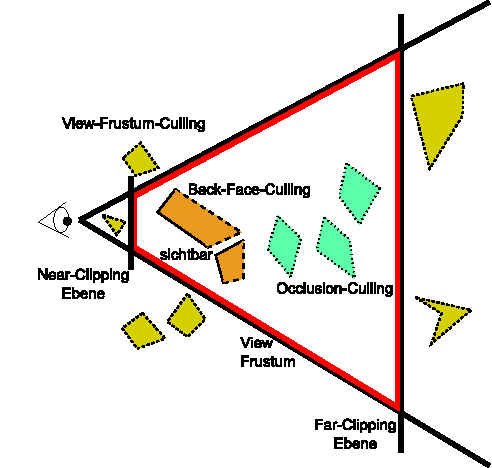
\includegraphics[scale=0.8]{images/culling.pdf}
  \caption{Verschiedene Culling-Techniken. Entfernte Geometrie ist durch gestrichelte Linien dargestellt. \textit{Quelle: nach \cite{culling}} }
  \label{fig:basics:culling}
\end{figure}
Beim Back-Face-Culling\footnote{\cite{RTR3}, Seiten 662 ff.} werden diejenigen Polygone entfernt, die vom Betrachter abgewandt sind. In Abbildung \ref{fig:basics:culling} würden bei den orangen Polygonen die vorderen Flächen gerendert, wobei die hinteren entfert würden (gestrichelte Linien). Dabei muss jede Fläche separat auf ihre Ausrichtung überprüft werden. In dieser Arbeit wird die von OpenGL angebotene Funktion für Back-Face-Culling verwendet.\\
View-Frustum-Culling entfernt Polygongruppen, die sich außerhalb des ViewFrustums befinden. In Abbildung \ref{fig:basics:culling} wären alle gelben Flächen außerhalb des Frustums (roter Bereich) davon betroffen. Alle Objekte, die sich vollständig oder partiell im Kamerabereich befinden, müssen gerendert werden. Da die Überprüfung von mehreren Millionen Dreiecken pro Frame zu teuer ist, werden lediglich die Boundingboxen von Objektgruppen getestet. Verwendet man zusätzliche räumliche Datenstrukturen, wie Octrees (siehe \ref{sec:basics:octree}), kann das Frustum-Culling hierarchisch durchgeführt werden. Dabei wird der Baum von der Wurzel bis zu dem Blättern durchlaufen. Liegt eine Boundingbox vollständig im Frustum, können alle Kindknoten ohne weitere Tests ebenfalls gezeichnet werden. Liegt eine Boundingbox vollständig außerhalb der Boundingbox, kann der Knoten samt aller Kindknoten entfernt werden, da diese ebenfalls außerhalb des Frustums liegen. Wird eine Box jedoch von einer Grenze des Frustums geschnitten, muss zum Einen die Geometrie im Knoten gerendert und die Kindknoten weiter getestet werden. Als weitere Möglichkeit zur Optimierung kann man sich diejenigen Grenzen speichern, die eine Box schneiden. Bei folgenden Tests der Kinder, müssen diese nur noch auf die gespeicherten Schnittflächen überprüft werden.\\
Soll vermieden werden, dass Objekte, die durch andere Polygongruppen verdeckt sind, gerendert werden, spricht man von Occlusion-Culling\footnote{\cite{RTR3}, Seiten 670 ff.}. Solche verdeckten Polygone würden in der Rendering-Pipeline transformiert, beleuchtet und anschließend gerastert, obwohl im fertigen Bild nicht davon sehen wäre. In Abbildung \ref{fig:basics:culling} sind die grünen Objekte vollständig verdeckt. Um mehrere Objekte auf ihre Sichtbarkeit zu überprüfen, wird gegen den Tiefenbuffer (Z-Buffer) getestet. Dazu muss schon ein Teil der Szene im Tiefenbuffer gerendert sein. Dabei ist die Zeichenreihenfolge wichtig. Gerendert wird in der Regel von vorne nach hinten in Abhängigkeit vom Standpunkt des Betrachters. Wird beispielweise bei der Boeing die Außenhülle als erstes gezeichnet, kann diese als Testgrundlage im Z-Buffer verwendet werden um das Innenleben, wird Letzteres wahrscheinlich nicht zu sehen sein. Dreht man die Reihenfolge um, müssen beide Teile gerendert werden. Entfernung von Objekten zur Kamera spielt ebenfalls eine Rolle. So kann eine Streichholzschachtel eine Golden Gate Bridge vollständig verdecken, wenn sich der Betrachter hinreichend dicht an der Streichholzschachtel befindet. Mittlerweile lässt sich Occlusion-Culling direkt auf der Grafik-Hardware durchführen. Dazu werden Occlusion-Queries verwendet, die nach dem Test ausgeben, wieviele Pixel der Objekte sichtbar sind. Dazu können vorher alle grafischen Effekte, wie Shader, Beleuchtung, usw, ausgeschaltet werden, um den Vorgang zu beschleunigen. Die Geschwindigkeit lässt sich noch verbessern, wenn statt der Originalgeometrie, nur Approximationen der Objekte gerendert werden. In dieser Arbeit wird Occlusion-Culling deshalb auf Boundingboxen durchgeführt. Dies kann jedoch zu falschen Testergebnissen führen. In Abbildung \ref{fig:basics:oculling} sind zwei verdeckte Objekte zu sehen. Beide befinden sich in der gleichen Boundingbox. Diese Box ist jedoch sichtbar und beide Objekte werden gerendert.

\todo[size=\small, inline]{Subsection-Titel ändern! Evtl. auch vorziehen bevor subsection Culling}
\subsection{Verschiedenes}
Das $c$-Collision Protokoll wird in Kapitel \ref{chap:relwork} genauer beschrieben. In dieser Arbeit wird es verwendet, um Datenanfragen möglichst gleichmäßig im Netzwerk zu verteilen. Jedes VBO (siehe \ref{sec:basics:computergrafik}) wird zufällig und redundant im Netzwerk verteilt. Alle Anfragen von allen Renderern werden jeden Frame gesammelt. Anschließend werden diese Anfragen zu Paketen gebündelt, die ebensoviele Anfragen enthalten wie es Datenknoten im Netzwerk gibt. Das $c$-Collision Protkoll wird immer auf einem Anfragenpaket ausgeführt. Begonnen wird  mit $c = 2$. Sollte in einer Runde kein weiterer Auftrag vergeben werden, obwohl noch offene Auftrage vorhanden sind, wird das $c$ erhöht. Dies wird so lange wiederholt, bis alle Aufträge vergeben sind.
\todo[size=\small, inline, color=magenta]{Kapitel: Algorithmen}

Da im Rahmen dieser Arbeit ein Sort-First-Renderer (siehe auch Kapitel \ref{chap:relwork}) entwickelt wurde, wurden zur Lastbalancierung der Renderknoten auch eine dynamische Kachelung implementiert.

Splittree (ähnlich KD-Baum nur mit Gewichtung)

\begin{figure}
  \centering
  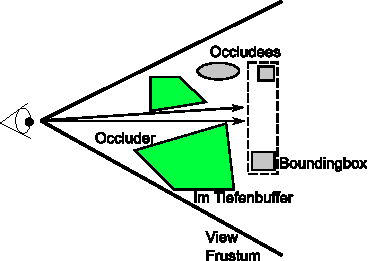
\includegraphics[scale=0.8]{images/oculling.pdf}
  \caption{Problem beim Occlusion Culling: Boundingbox zweier Objekte ist sichtbar, obwohl die darin enthaltenen Objekte verdeckt sind.}
  \label{fig:basics:oculling}
\end{figure}

\subsection{Caching}
\label{sec:basics:caching}
\todo[size=\small, inline, color=blue!40]{Kapitel: Caching}
\begin{itemize}
  \item wird über Algos gefüllt
  \item extendedFrustum / PreFetching 
\end{itemize}

\subsection{Speichermanagement}
\label{sec:basics:speichermanagement}
\todo[size=\small, inline, color=blue!40]{Kapitel: Speichermanagement}
\begin{itemize}
 \item nicht jeder braucht alles -> Kacheln
 \item Gewichtung über die Anzahl der Dreiecke pro Request
\end{itemize}

\section{Approximation}
\label{sec:basics:approximation}
\todo[size=\small, inline, color=blue!40]{Unterkapitel: Approximation}
Approximationen in der Computergrafik haben oft  Zurfolge, dass die Bildqualität verringert wird. Sei es weil Objekte in niedrigeren Auflösungen
\begin{itemize}
 \item Occlusion-Culling entfernt teile
 \item Nicht immer sofort ein vollständiges Bild verfügbar -> nach und nach nachladen
 \item Teile können weggelassen werden $\rightarrow$ OcclusionCulling \& FrustumCulling
 \item Begrenzung des Cache-Kontingents
 \item Tiefenbuffer Update nur alle paar Frames
 \item Sampletree
\end{itemize}

\chapter{Versuchsaufbau}
\section{Das Programm}

\label{masternode}
MasterNode:
\begin{itemize}
 \item verschicke Kameraposition und Tasteneingabe
 \item warte auf Objektanfragen von allen RenderNodes
 \item führe c-Collision Protokoll auf diesen aus, gebündelt zu Anfrangen der Menge an DataNodes
 \item sende die Anfragen an die ausgewählten DataNodes weiter
 \item warte auf Kacheln von allen RenderNodes
\end{itemize}

\label{rendernode}
RenderNode:
\begin{itemize}
 \item warte auf Tasteneingaben und Kameraposition
 \item Erweitere das Frustum und parse den Octree/Sampletree
 \item Jeder Knoten im Frustum bekommt einen Zeitstempel
 \item sollte ein Knoten schon länger online oder offline sein, tagge den Knoten für eine erneute Überbprüfung.
 \item schicke Anfragen über fehlende Objekte an den MasterNode
 \item Rendere eine Kachel mit allen verfügbaren Knoten, die online sind.
 \item Beginne Empfang aller anstehenden Knoten.
 \item verschicke die Kachel an den MasterNode
\end{itemize}

\label{datanode}
DataNode:
\begin{itemize}
 \item warte auf irgendeine ankommende Nachricht
 \item Ist es ein Request, sortiere die Requests nach RenderNode und beginne mit den Occlusion-Tests
 \item Bei erfolgreichen Tests wird das Objekt vollständig in den Tiefenbuffer gerendert
 \item Verschicke alle positiv getesteten Objekte an die anfordernden RenderNodes
 \item Ist es ein Tiefenbuffer, schreibe den Buffer für den jeweiligen RenderNode in den FrameBuffer
\end{itemize}


\chapter{Evaluierung}
\label{chap:eval}
\todo[size=\small, inline]{Walkthrough-Pfad noch einfügen hier}%
\todo[size=\small, color=yellow!40, inline]{Needs Non-Tim understanding}%
\todo[size=\small, color=yellow!40, inline]{Needs Human proofreading}%

Um die Effektivität des in dieser Arbeit entstandenen Systems überprüfen zu können, wurden verschiedene Tests durchgeführt.
Beim ersten Test, dem \textit{FPS-Test}, wurde die gemessene Bildrate bei einem Walkthrough\footnote{\todo[size=\small,inline]{Walkthrough-Erklärung an erste Stelle des Auftauchens innerhalb der Arbeit schieben. Vermutlich Intro.}Ein Walkthrough bezeichnet hier eine Navigation durch eine 3D-Szene, bei der möglichst viele signifikante Stellen des Modells besucht werden.} durch die Szene aufgezeichnet. Der \textit{Reload-Test} hat bei verschiedenen Systemkonfigurationen an festen Kamerapositionen die Zeit gemessen, die ein erneutes Laden der Szene benötigt. Beim \textit{$c$-Collision-Test} wurde die Last der einzelnen Datenknoten während eines Walkthroughs gemessen. Die einzelnen Testläufe unterscheiden sich dabei in der verwendeten Anzahl an Datenknoten und Redundanzen. Redundanz bedeutet hier, wie oft das Modell der Boeing vollständig im Netzwerk verteilt wurde. \\
Zur Entwicklung des Systems wurde ein kleinerer Cluster benutzt, bestehend aus 8 Pentium Multicore-Rechnern in einem Gigabit Netzwerk, sowie einem Quadcore-Pentium mit einer GeForce 260GTX Grafikkarte als Render- und Masterknoten, im Folgenden \textit{Entwicklungs-Cluster} genannt. Die eigentlichen Tests erfolgten auf dem Arminius-Cluster des PC$^2$s (siehe Tabelle \ref{tab:impl:arminius}).\\
Im Arminius-Cluster wurde der Compiler gcc 3.4.6, OpenGL als Grafik-API, nVidia Treiber v177 auf den Rechenknoten und v190 auf den Visualisierungsknoten benutzt, sowie die boost-Bibliothek v1.38 und OpenMPI v1.2.9. Die Auflösung betrug jeweils 640$\times$480 Pixel für das normale Frustum und 800$\times$600 Pixel für das erweiterte Frustum.\\
Zusätzliche Diagramme und Abbildungen sind in den Anhängen \ref{chap:add_diag} und \ref{chap:add_fig} zu finden.

\section{FPS-Test}
\label{sec:eval:fps}
Bei diesem Test wurde in einem festgelegten Walkthrough durch die 3D-Szene gemessen, wie viele Bilder pro Sekunde an welcher Stelle der Szene erreicht werden konnten. Dazu wurde der Walkthrough auf je 24, 28 und 32 Datenknoten mit einer Redundanz von 1, 2 und 3 durchgeführt. Die y-Achsen der Diagramme in Abbildung \ref{fig:eval:fps} stellen die Bilder pro Sekunde dar und die x-Achsen die Messpunkte während des Walkthroughs. Die FPS jeden Frame darzustellen ist nicht praktikabel, da diese stark schwanken. Daher wurden die gemessenen FPS in diesem Test jeweils über 20 Frames gemittelt.
\begin{figure}
\centering
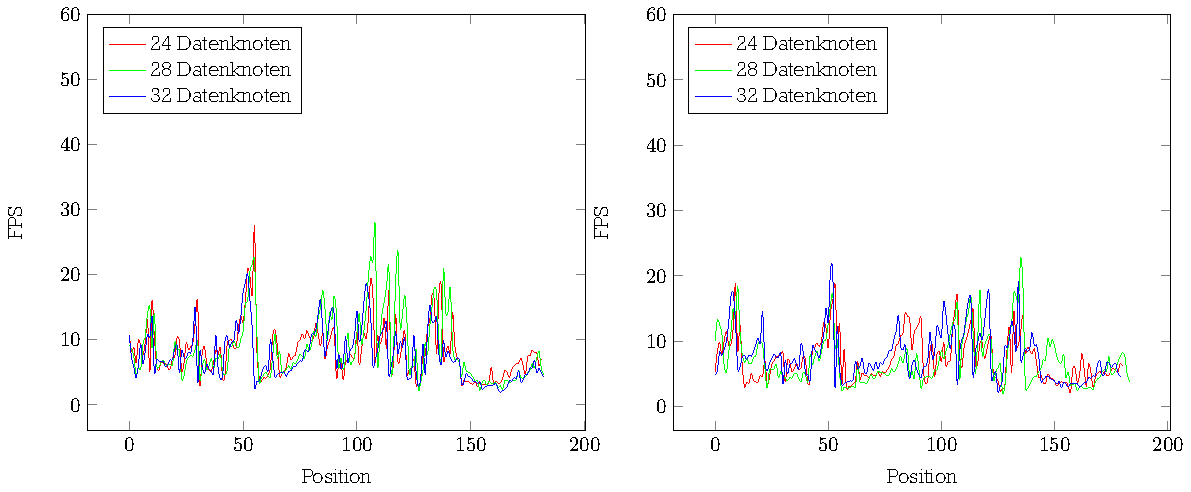
\includegraphics[scale=0.75]{images/diag_fps.pdf}
  \caption{\label{fig:eval:fps}FPS in einem Walkthrough mit 4 Renderknoten und 24-32 Datenknoten. \textit{links: Redundanz$=$1; rechts: Redundanz$=$3.}}
\end{figure}

An den Diagrammen kann man sehen, dass sich die Bildrate bei verschiedenen Konfigurationen ähnelt. Allerdings lassen sich keine Zusammenhänge zwischen Bildrate und Redundanz oder Knotenanzahl herstellen. Die Bildrate gibt eher Rückschlüsse darauf, wie die Szene an den einzelnen Positionen beschaffen ist. An Stellen des Modells, wo sehr viel Geometrie angefordert werden muss, ist die Bildrate vermutlich geringer, als an Stellen, an denen weniger angefordert wird. Hinzu kommt der Umstand, dass die Grafikkarten der Datenknoten im hier verwendeten Arminius-Cluster, nicht sehr leistungsstark sind. In Testumgebungen mit aktuellerer Grafikhardware würde die Zahl der Redundanzen und der Knoten möglicherweise stärker ins Gewicht fallen. Trotz geringerer Netzwerk-Bandbreite konnten im \textit{Entwicklungs-Cluster} teilweise höhere FPS gemessen werden, als im Arminius-Cluster. Beim gleichen Walkthrough auf dem \textit{Entwicklungs-Cluster} zeigte sich, dass nach kurzer Zeit kaum noch Objekte dargestellt wurden. Durch die kontinuierliche Bewegung wird der Tiefenbuffer alle 20 Frames aktualisiert, was zur Folge hat, dass alle laufenden Aufträge verworfen werden. In dem langsameren Netzwerk kamen dadurch kaum noch Objekte bei den Renderknoten an. Die Geschwindigkeit des verwendeten Netzwerks hat somit Auswirkungen auf die Bildqualität.

\section{Reload-Test}
\label{sec:eval:reload}
Beim Reload-Test wurde an festgelegten Kamerapositionen gemessen, wie lange die einzelnen Datenknoten benötigen, um die für diese Szene anfallenden Aufträge vollständig zu bearbeiten. Dazu wurden sämtliche auf den Renderern befindlichen Objekte verworfen und erneut angefordert. War ein Datenknoten mit der Bearbeitung aller Aufträge fertig, hat er sich beim Masterknoten zurückgemeldet und die gemessene Zeit wurde gespeichert.
\begin{figure}
\centering
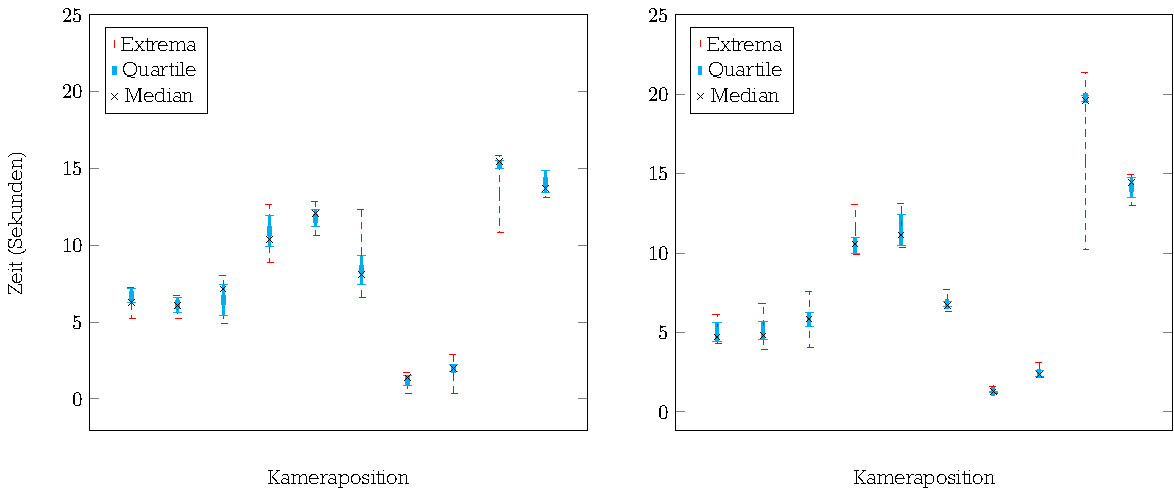
\includegraphics[scale=0.75]{images/diag_reload.pdf}
  \caption{\label{fig:eval:reload}Reload-Test mit 2 Renderknoten: \textit{links: Redundanz 1 und 24 Renderknoten; rechts: Redundanz 3 und 32 Renderknoten}.}
\end{figure}
Die Diagramme in Abbildung \ref{fig:eval:reload} enthalten auf den x-Achsen die Kameraposition und auf den y-Achsen die Render-Zeit in Sekunden. In den Diagrammen ist zu erkennen, dass der Median meist nahe am Durchschnitt liegt. Die Messungen wurden dabei mehrfach durchgeführt und die Ergebnisse wurden gemittelt. Ab und zu sind zwar einige Ausreißer zu erkennen, aber selbst die 0.25 und 0.75 Quantile liegen meist sehr dicht am Median. Das bedeutet, dass das System gut balanciert. Nur wenige Knoten benötigen mehr Zeit zum Rendern ihrer Aufträge, als das beim Median der Fall ist. Jedoch lässt auch dieser Test keinen Zusammenhang zwischen Redundanzen, Knotenanzahl und der benötigten Zeit erkennen. Die Beschaffenheit der Szene an einer gegebenen Kameraposition scheint ausschlaggebend für die gesamte benötigte Bearbeitungszeit zu sein. Mehr Geometrie an einer Position bedeutet auch mehr zu vergebene Aufträge, was mehr Zeit in Anspruch nimmt, als das bei weniger Geometrie der Fall ist. In den Abbildungen \ref{fig:eval:pos3} und \ref{fig:eval:pos5} finden sich Screenshots von zwei exemplarischen Kamerapositionen. Zusätzliche Screenshots sind im Anhang \ref{chap:add_fig} zu finden.
\begin{figure}
\centering
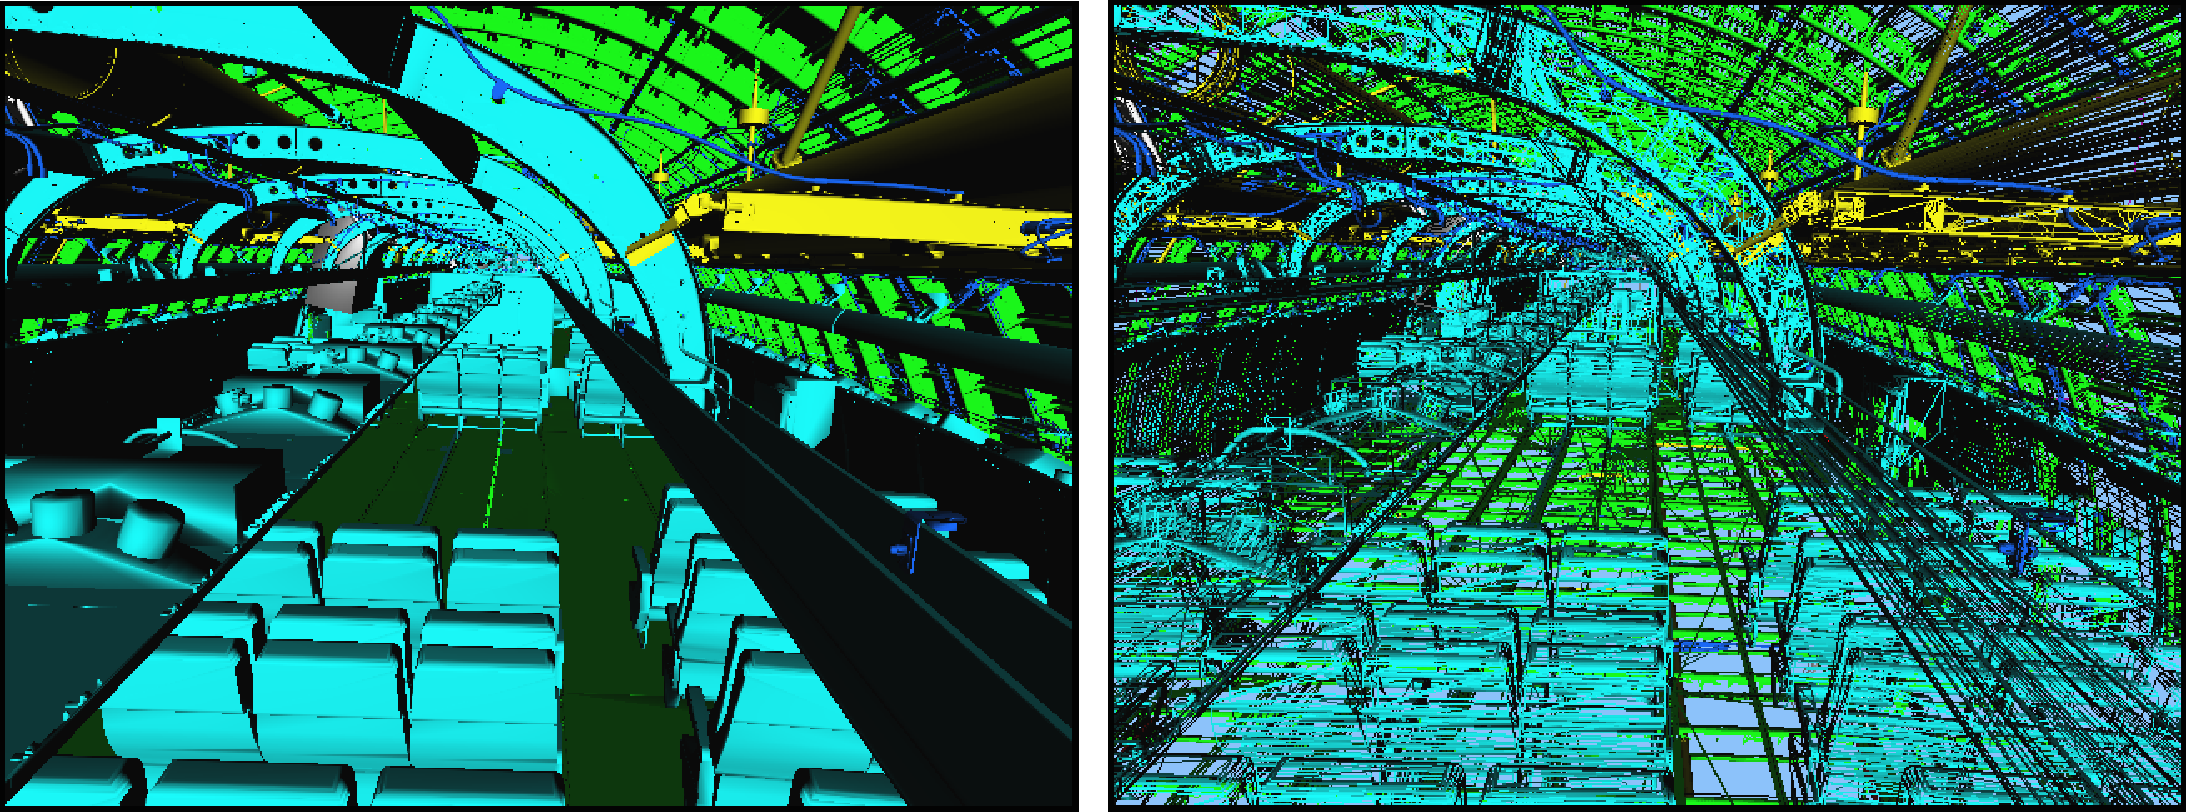
\includegraphics[scale=0.40]{images/pos3.pdf}
\caption{\label{fig:eval:pos3}Kameraposition 3: \textit{links: die Szene im normalen Rendering-Modus; rechts: die Szene im Gitternetz-Modus (Passagierbereich, 3.749.977 sichtbare Dreiecke).}}
\end{figure}

\begin{figure}
\centering
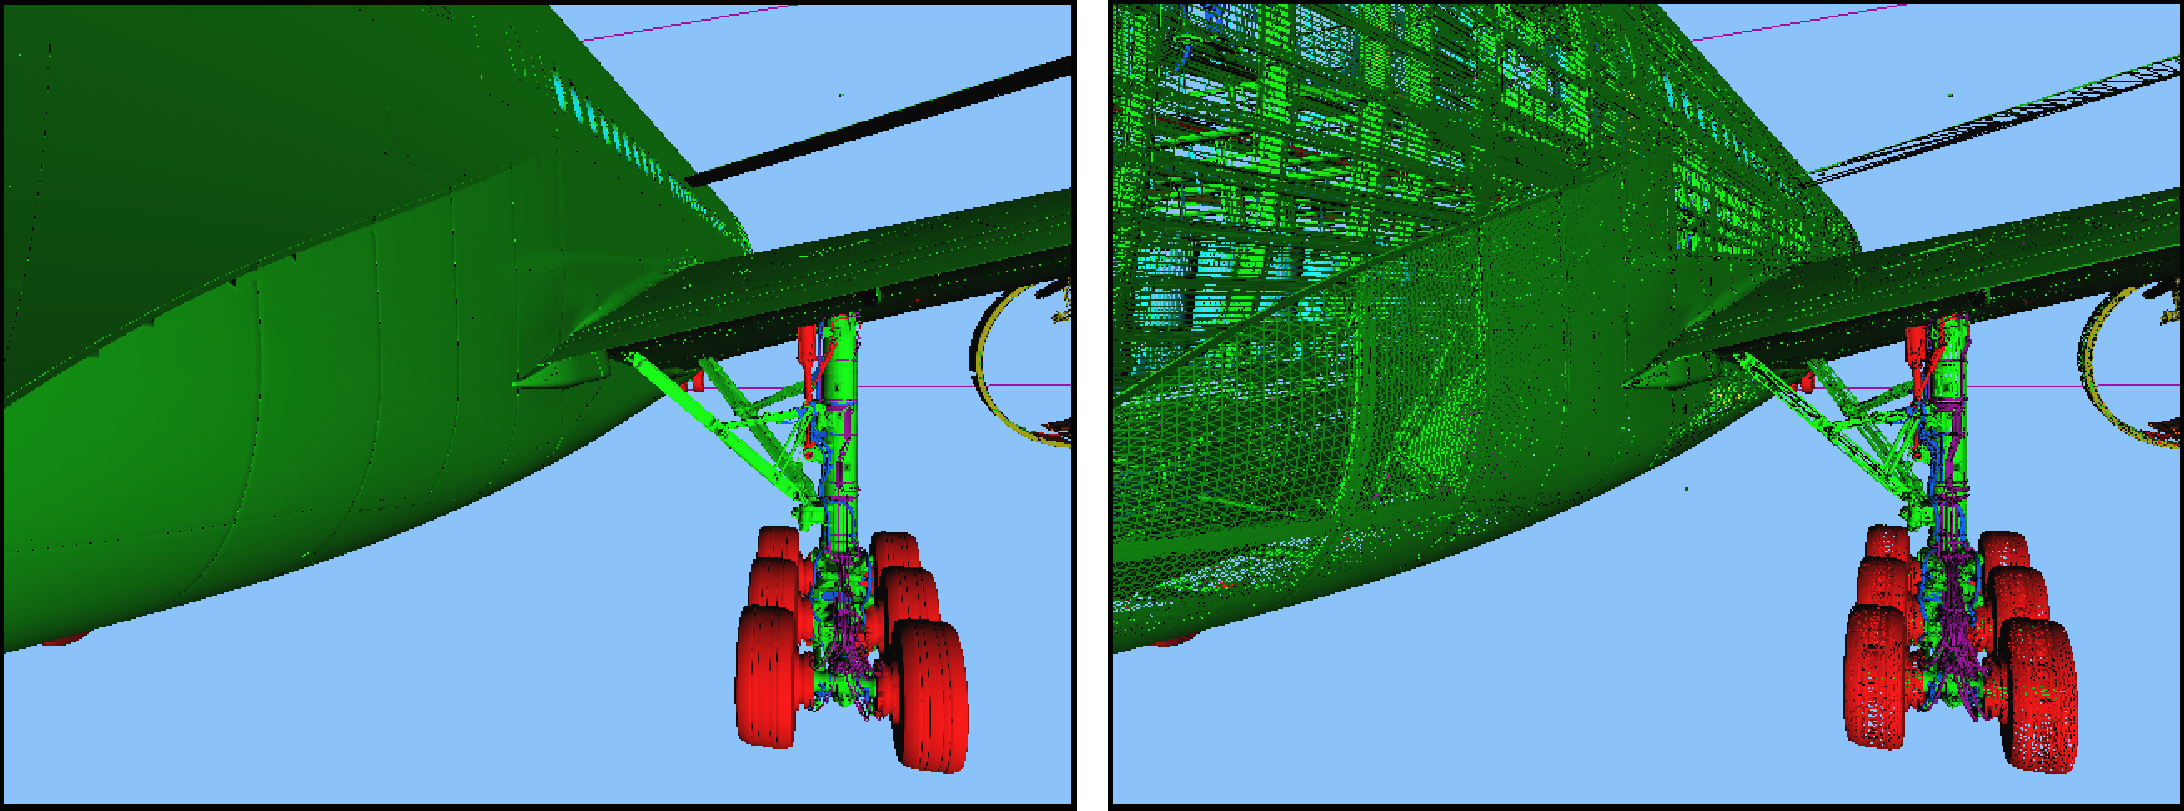
\includegraphics[scale=0.40]{images/pos5.pdf}
\caption{\label{fig:eval:pos5}Kameraposition 5 \textit{links: die Szene im normalen Rendering-Modus; rechts: die Szene im Gitternetz-Modus (Fahrwerk/Flügel, 5.776.159 sichtbare Dreiecke).}}
\end{figure}

\section{\textit{c}-Collision-Test}
\label{sec:eval:ccollision}

Der Test für das $c$-Collision Protokoll wurde als Einziger nicht im Cluster durchgeführt, sondern ausschließlich in einer Simulation. Dafür wurden alle Anfragen bei einem tatsächlichen Walkthrough durch die Szene aufgezeichnet, unmittelbar bevor sie durch das $c$-Collision Protokoll vergeben wurden. Anschließend wurden diese Aufzeichnungen genutzt, um eine beliebige Datenknotenmenge zu simulieren. Im Arminius-Cluster standen für diese Arbeit maximal 2 Visualisierungsknoten und 32 Datenknoten zur Verfügung, weshalb die Menge der Datenknoten in dieser Simulation erhöht wurde. Andere Mengen an Renderknoten lassen sich nicht ohne Weiteres simulieren, da die Renderknoten bestimmen, wann welche Objekte benötigt werden. Deshalb sind keine realistischen Aussagen über Anfragefolgen bei künstlich veränderter Renderknotenmenge möglich.\\
In diesem Test wurden 24, 80 und 120 Datenknoten simuliert. Dabei wurde die Last in Form von Dreiecken gemessen, die in jedem Frame an jeden Datenknoten vergeben wurde. In diesem Test wurden verschiedene Zufalls-Seeds benutzt und das Ergebnis wurde gemittelt.
\begin{figure}
\centering
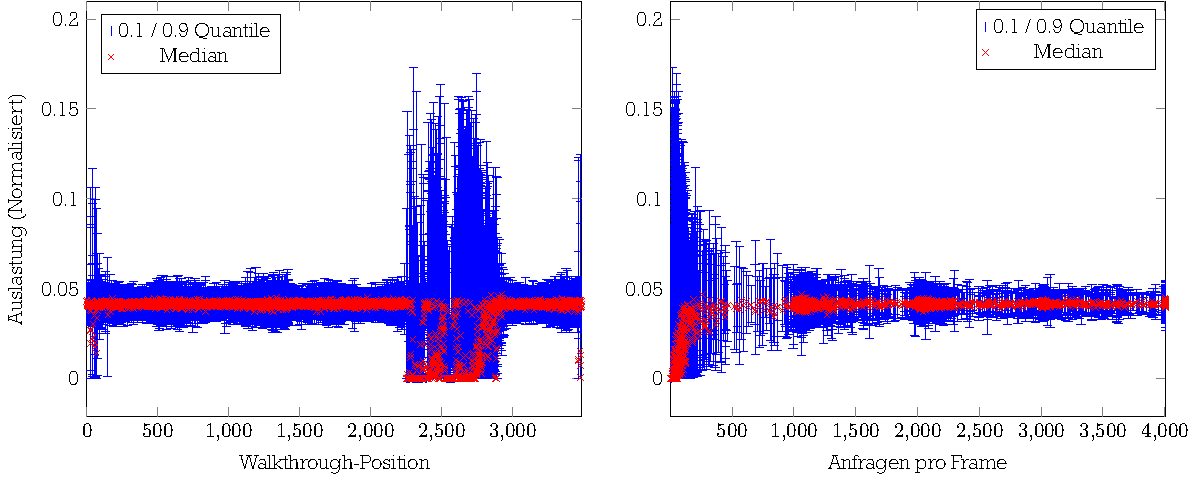
\includegraphics[scale=0.75]{images/diag_cCol_red1_render4_data24_2x.pdf}
  \caption{\label{fig:eval:cCol1}Die Auslastung der Datenknoten in einem Walkthrough bei 4 Renderknoten und 24 Datenknoten und Redundanz$=$1.}
\end{figure}

In den Abbildungen \ref{fig:eval:cCol1} und \ref{fig:eval:cCol9} zeigt das linke Diagramm jeweils die Walkthrough-Position (x-Achse) in Relation zur Lastverteilung (y-Achse). Das rechte Diagramm zeigt jeweils die Anfragenmenge, die durch das $c$-Collision Protokoll pro Frame verteilt wurde (x-Achse), in Relation zur Lastverteilung (y-Achse). In Abbildung \ref{fig:eval:cCol1} wurden 24 Datenknoten mit einer Redundanz von 1 simuliert, in Abbildung \ref{fig:eval:cCol9} wurden 120 Datenknoten mit einer Redundanz von 3 simuliert. Bei Betrachtung des linken Diagramms fallen einige Positionen auf, an denen die Last sehr ungleich verteilt ist oder der Median 0 ist. Im rechten Diagramm kann man sehen, dass dies immer dann der Fall ist, wenn das c-Collision Protkoll sehr wenige Anfragen verteilen musste. Dieses Protokoll dient ursprünglich dazu, Bälle möglichst gleichmäßig auf Körbe zu verteilen. Hat man viel weniger Bälle als Körbe, ist das System nicht gleichmäßig balanciert, da einige Körbe gar keine Bälle erhalten. Sowie die Bälle sind auch die Anfragen im Test-System atomar und werden nicht weiter unterteilt. Je nach initialer Zufallsverteilung der Daten auf den Knoten, kann es bei wenig Redundanzen auch vorkommen, dass die Aufträge nur auf wenige Knoten verteilt werden können. Im Falle des benutzen Walkthroughs, treten die unbalancierten Stellen da auf, wo das Model betreten und verlassen wird. An diesen Stellen gibt es sehr wenig sichtbare Geometrie.\\
Bei diesem Test ist zu erkennen, dass sowohl die Menge an Knoten als auch die Zahl der Redundanzen eine Rolle bei der gleichmäßigen Lastverteilung spielt. Bei erhöhter Redundanz ist zu beobachten, dass die 0.1 und 0.9 Quantile sehr viel näher am Median liegen als bei geringerer Redundanz. Mehr Datenknoten sorgen dafür, dass die Spitzenwerte an unbalancierten Stellen geringer ausfallen.
\begin{Bild}
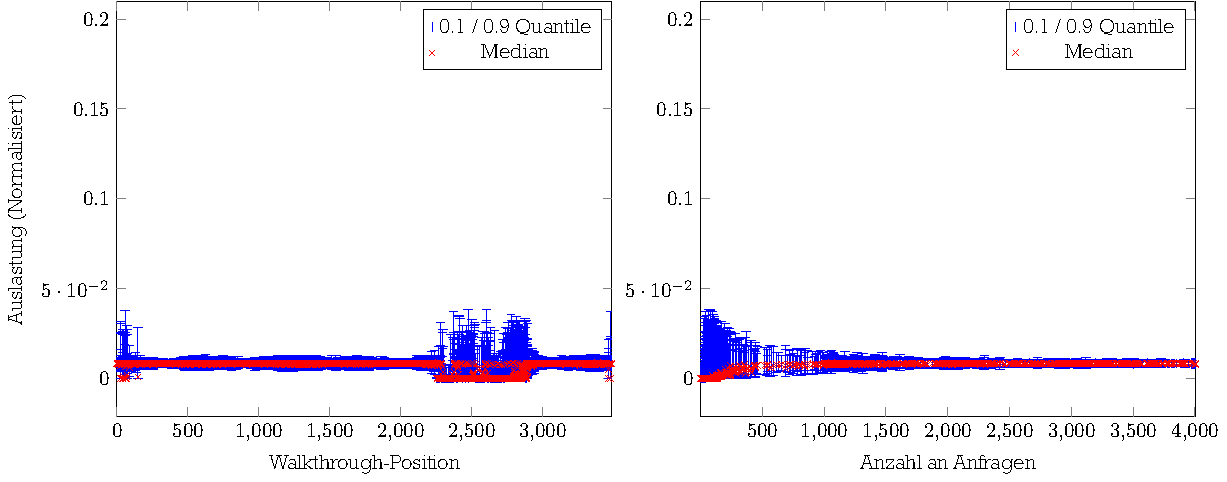
\includegraphics[scale=0.75]{images/diag_cCol_red3_render4_data120_2x.pdf}
  \captionof{figure}{\label{fig:eval:cCol9}Die Auslastung der Datenknoten in einem Walkthrough bei 4 Renderknoten und 120 Datenknoten und Redundanz$=$3.}
\end{Bild}


%  ----------------------------------------------------------------------------
%
%       Copyright (for the thesis) 2009 by [author - insert yourself]
%
%       This thesis is published under the
%       Creative Commons Attribution-No Derivative Works 3.0 Austria License
%       as detailed at http://creativecommons.org/licenses/by-nd/3.0/at/
%
%  ----------------------------------------------------------------------------
%  Template credits and license:
%  ----------------------------------------------------------------------------
%
%       "Fakultät für Informatik" diploma/master thesis template 2008
%
%       based upon "Diploma thesis template 2005" by lukas.silberbauer(at)gmx.at
%       based upon "Diplomarbeit mit LaTeX" by Tobias Erbsland
%       incorporating a title page by Informatik-Forum user "Baby"
%       polished and ported to the TU fonts package by Jakob Petsovits
%
%       published under the terms of
%
%  ----------------------------------------------------------------------------
%  "THE BEER-WARE LICENSE":
%  <lukas.silberbauer(at)gmx.at> wrote this file. As long as you retain this
%  notice you can do whatever you want with this stuff. If we meet some day,
%  and you think this stuff is worth it, you can buy me (us) a beer in return.
%  ----------------------------------------------------------------------------
%
%  (end of template credits)
%

\chapter{Fazit und Ausblick}
\label{conclusion}

Ausblick:
\begin{itemize}
 \item Mechanismen zur Bildkonpression verwenden bevor RGB- oder Tiefen-Informationen verschickt werden.
  \item Ankündigung des Bedarfs an günstigen Approximationen für Backend-Knoten $\rightarrow$ Verweis auf Clemens
\end{itemize}

%
% EOF
%


\appendix

%  ----------------------------------------------------------------------------
%
%       Copyright (for the thesis) 2009 by [author - insert yourself]
%
%       This thesis is published under the
%       Creative Commons Attribution-No Derivative Works 3.0 Austria License
%       as detailed at http://creativecommons.org/licenses/by-nd/3.0/at/
%
%  ----------------------------------------------------------------------------
%  Template credits and license:
%  ----------------------------------------------------------------------------
%
%       "Fakultät für Informatik" diploma/master thesis template 2008
%
%       based upon "Diploma thesis template 2005" by lukas.silberbauer(at)gmx.at
%       based upon "Diplomarbeit mit LaTeX" by Tobias Erbsland
%       incorporating a title page by Informatik-Forum user "Baby"
%       polished and ported to the TU fonts package by Jakob Petsovits
%
%       published under the terms of
%
%  ----------------------------------------------------------------------------
%  "THE BEER-WARE LICENSE":
%  <lukas.silberbauer(at)gmx.at> wrote this file. As long as you retain this
%  notice you can do whatever you want with this stuff. If we meet some day,
%  and you think this stuff is worth it, you can buy me (us) a beer in return.
%  ----------------------------------------------------------------------------
%
%  (end of template credits)
%

\chapter{Glossar}

\begin{acronym}
\acro{API}{Application Programming Interface}
\acro{CAD}{Computer Aided Design}
\acro{CPU}{Central Processing Unit (Hauptprozessor)}
\acro{FPS}{Frames per second}
\acro{GPU}{Graphics Processing Unit (Grafikprozessor)}
\acro{HLOD}{Hierarchical Level-Of-Detail \cite{hlod}}
\acro{KD-Baum}{Ein k-dimensionaler Baum oder KD-Baum ist ein unbalancierter Suchbaum zur Speicherung von Punkten. (siehe \cite{RTR3}, Seite 650 ff.)}
\acro{LOD}{Level-Of-Detail (siehe \cite{RTR3}, Seite 680 ff.)}
\acro{PLP}{Prioritized-Layered Projection \cite{plp}}
\acro{Octree}{Ein Octree ist eine räumliche Datenstruktur, bestehend aus einem gewurzelten Baum, dessen Knoten jeweils entweder acht direkte Nachfolger oder gar keine Nachfolger haben.}
\acro{peer-to-peer}{Peer-to-peer Netzwerke sind Netzwerksysteme ohne zentrale Zugriffskontrolle, in denen alle Rechner gleichberechtigt agieren. Eine Datenverbindung besteht dabei immer direkt von einem Teilnehmer zum anderen.}
\acro{PVS}{Potentially Visible Set (siehe \cite{RTR3}, Seite 660 ff.)}
\acro{Quantil}{Ein $p$-Quantil ist ein Lagemaß in der Statistik, wobei $p$ eine reelle Zahl zwischen 0 und 1 ist. Das $p$-Quantil ist ein Merkmalswert, der die Verteilung einer Variablen bzw. Zufallsvariablen in zwei Teile teilt. Links vom $p$-Quantil liegen $100\cdot p$ Prozent aller Beobachtungswerte bzw. $100\cdot p$ Prozent der Masse der Zufallsvariablen. Rechts davon liegen $100\cdot(1-p)$ Prozent aller Beobachtungswerte bzw. $100\cdot(1-p)$ Prozent der Masse der Zufallsvariablen.}
\acro{Quartil}{Quartile sind die Quantile 0,25-Quantil, 0,5-Quantil=Median und 0,75-Quantil.}
\acro{Rasterisierung}{Überführung eines kontinuierlichen Raums in einen diskreten Raum (Pixel).}
\acro{Rendering}{Erzeugt ein 2D-Bild aus einer 3D-Szene.}
\acro{screen-space}{Projektion einer 3D-Szene in einen zweidimensionalen Raum (Bild).}
\acro{SGI}{SGI ist ein Hersteller von Computern, die besonders auf dem Gebiet der grafischen Darstellung leistungsstark sind (Grafik-Workstation).}
\acro{SLI}{Scalable Link Interface; Zusammenschluss mehrer Grafikchips}
\acro{View-Frustum}{Sichtfeld der Kamera}
\end{acronym}

%
% EOF
%


\bibliographystyle{alpha}
\bibliography{bib/references}

%\printindex
\end{document}

%
% EOF
%
